% ~ 12 pages
\chapter{Identification of Hadronically Decaying $\tau$-Leptons (NN)}
\label{sec:rnn}

\section{Identification using Feedforward Neural Networks}
\label{sec:ffnn_id}

\begin{itemize}
\item MLP Tau-ID (only densely connected layers)
  \begin{itemize}
  \item Comparison with BDT-based ID
  \item Scaling with more data
  \end{itemize}
\end{itemize}

\section{Identification using Recurrent Neural Networks}
\label{sec:rnn_id}

\subsection{General Description}
\label{sec:rnn_descr}

State that the RNN is mainly optimised for 1-prong operation and give reasons
for that (i.e.\ higher branching ratio)

\subsection{Track-RNN}
\label{sec:rnn_tracks}

\todo{Choice of $z_0 \sin\theta$ instead of $z_0$ is due to expected larger
  error in forward direction}

\todo{Lower threshold for $p_\mathrm{T}$ is \SI{400}{\mega\electronvolt} already
  in track reconstruction}

\todo{use 10 tracks}

\todo{LSTM cell size scan? 8, 12, 16, 24, 32, 48, 64}

\begin{figure}[ht]
  \begin{subfigure}[t]{0.48\textwidth}
    \centering
    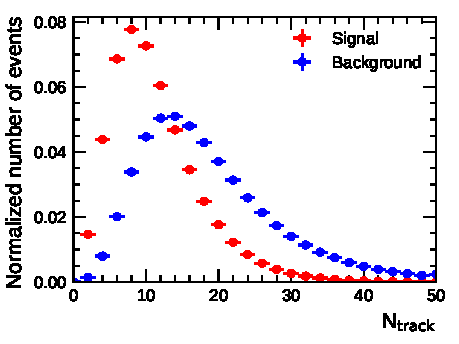
\includegraphics{./figures/rnn/ntrk_1p.pdf}
    \subcaption{NTracks for 1-prong taus.}
  \end{subfigure}\hfill
  \begin{subfigure}[t]{0.48\textwidth}
    \centering
    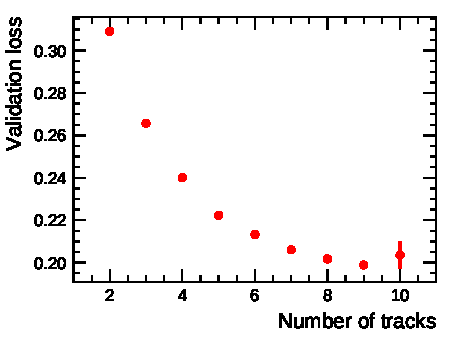
\includegraphics{./figures/rnn/nscan/track_1p.pdf}
    \subcaption{Val.\ loss vs.\ nTracks. Also put 3P in this? Errors are of the
      order of the marker size.}
  \end{subfigure}
  \caption{Tracks associated with a tau}
  \label{fig:rnn_ntracks}
\end{figure}

\begin{itemize}
\item Motivation (i.e. \texttt{SumPtTrkFrac} \& MVA-tracking)
\item Architecture (mention rough optimisation by hand while monitoring
  validation loss)
\item Preprocessing
\item Input variables \& correlation with true (or predicted?) class labels.
  Partial dependence plots? Variable importance?
\item Validation loss vs. number of tracks
\item Standalone performance vs. BDT-based ID
\end{itemize}

\begin{itemize}
\item Replace $\Delta R_\mathrm{JS}$ with $\Delta \eta$ and $\Delta \varphi$
  (try extrapolated \& non-extrapolated)
\item Replace pt asymmetry with $pt_\mathrm{JS}$
\item Do a validation loss vs.\ number of tracks scan
\item Validation loss vs.\ sample size
\end{itemize}

\subsection{Cluster-RNN}
\label{sec:rnn_clusters}

\begin{figure}[ht]
  \begin{subfigure}[t]{0.48\textwidth}
    \centering
    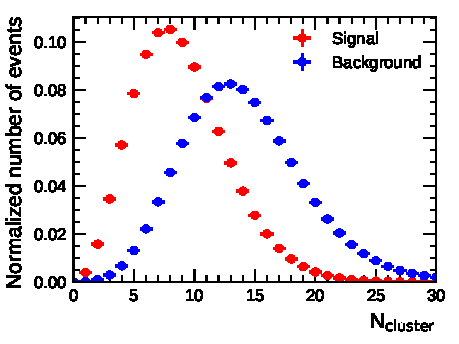
\includegraphics{./figures/rnn/ncls_1p.pdf}
    \subcaption{NCluster for 1-prong taus}
  \end{subfigure}%
  \begin{subfigure}[t]{0.48\textwidth}
    \centering
    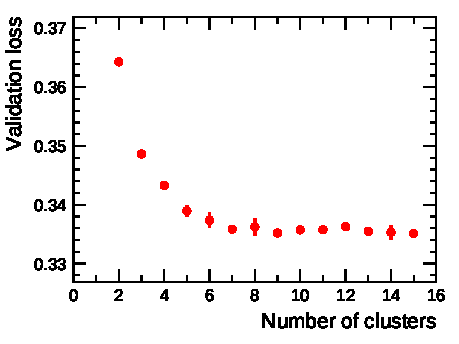
\includegraphics{./figures/rnn/nscan/cluster_1p.pdf}
    \subcaption{Val.\ loss vs.\ nCluster}
  \end{subfigure}
  \caption{Clusters associated with a tau}
  \label{fig:rnn_nclusters}
\end{figure}

\todo{Use 6 clusters}

\begin{itemize}
\item Input variables \& correlation with true class labels. Partial
  dependence plots?
\item Validation loss vs. number of clusters
\item Standalone performance
\end{itemize}

\subsubsection{Rate-Reduction at the High Level Trigger}
\label{sec:hlt_rate_reduction}

The high rates of the High Level Trigger (HLT) for tau leptons need to be
reduced. At the HLT no track information is available due to the high time
requirements of the ATLAS tracking algorithm. The rate reduction is limited to
calorimeter-based variables.

\subsection{Combined-RNN}
\label{sec:rnn_combined}



\begin{itemize}
\item Architecture
\item Performance w.r.t. BDT-ID
\end{itemize}


%%% Local Variables:
%%% mode: latex
%%% TeX-master: "mythesis"
%%% End:
